\documentclass{standalone}


\usepackage{tikz}
\usetikzlibrary{shapes.geometric, arrows}
\usetikzlibrary{positioning}


\tikzstyle{startstop} = [rectangle, rounded corners, minimum width=2cm, minimum
height=0.5cm,text centered, draw=black]

\tikzstyle{io} = [trapezium, trapezium left angle=70, trapezium right angle=110, minimum
width=2.5cm, minimum height=0.5cm, text centered, text width = 1.5cm, draw=black]

\tikzstyle{process} = [rectangle, minimum width=2cm, minimum height=0.5cm, text centered,
text width = 1cm, draw=black]
\tikzstyle{decision} = [diamond, minimum width=2cm, minimum height=0.5cm, text centered,
draw=black]

\tikzstyle{block1} = [rectangle, rounded corners, minimum width=0.5cm, minimum
height=0.25cm,text centered, draw=black]

\tikzstyle{block2} = [rectangle, rounded corners, minimum width=2.5cm, minimum
height=3.6cm,text centered, draw=black]



\tikzstyle{arrow} = [thick,->,>=stealth]

       
\usetikzlibrary{calc}   
\begin{document}

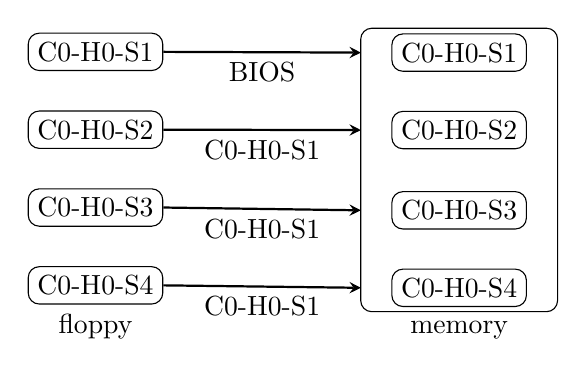
\begin{tikzpicture}[node distance=0.5cm]
  \node (C0-H0-S1f) [block1] {C0-H0-S1};
  \node (C0-H0-S2f) [block1, below=of C0-H0-S1f] {C0-H0-S2};
  \node (C0-H0-S3f) [block1, below=of C0-H0-S2f] {C0-H0-S3};
  \node (C0-H0-S4f) [block1, below=of C0-H0-S3f, label=below: floppy] {C0-H0-S4};
  \node (memory) [block2, right=of C0-H0-S1f, yshift=-1.5cm, xshift=2cm, label=below: memory] {};
  \node (C0-H0-S1) [block1] at ([yshift=-0.9em]memory.north) {C0-H0-S1};
  \node (C0-H0-S2) [block1] at ([yshift=-3.7em]memory.north) {C0-H0-S2};
  \node (C0-H0-S3) [block1] at ([yshift=-6.6em]memory.north) {C0-H0-S3};
  \node (C0-H0-S4) [block1] at ([yshift=-9.4em]memory.north) {C0-H0-S4};

  \draw[thick, ->, >=stealth] (C0-H0-S1f.east) to node [auto,swap] {BIOS} ($(C0-H0-S1.west) + (-1.1em,
  0)$);

  \draw[thick, ->, >=stealth] (C0-H0-S2f.east) to node [auto, swap] {C0-H0-S1}
  ($(C0-H0-S2.west) + (-1.1em, 0)$);

  \draw[thick, ->, >=stealth] (C0-H0-S3f.east) to node [auto, swap] {C0-H0-S1}
  ($(C0-H0-S3.west) + (-1.1em, 0)$);

  \draw[thick, ->, >=stealth] (C0-H0-S4f.east) to node [auto, swap] {C0-H0-S1}
  ($(C0-H0-S4.west) + (-1.1em, 0)$);
  
\end{tikzpicture}

\end{document}

%%% Local Variables:
%%% mode: latex
%%% TeX-master: t
%%% End:
